
\chapter{Field Tests}\label{ch:field_test}

Computer Vision algorithms can only give as good result as the source videostream that it is 
being fed. After talking a bit to \gls{sintef}, some test videos were provided by them. However, as seen in figure 
\vref{fig:sintef_not_1}, the quality leaves much to be desired. The video provided had a resolution 
of $854 \times 480$ pixels with big black box padding around it. This does not only make 
the video unsuitable for us in a computer vision algorithm, but it also means that the video 
probably is upscaled quite a bit.

Due to the poor nature of the quality of the video it was decided early on that 
a field test was needed, since we were going to use equivalent hardware as to what is available on the \gls{rov}. 

\begin{figure}[htbp]
	\centering
	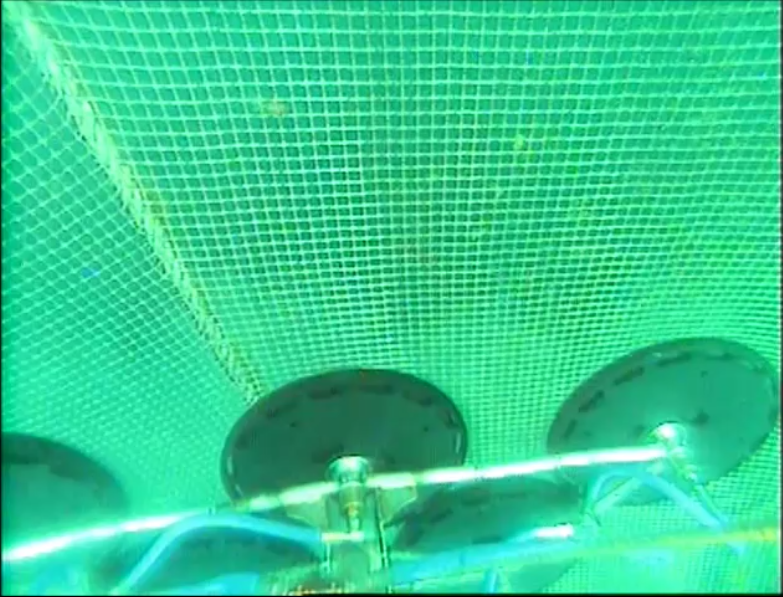
\includegraphics[width=0.9\textwidth]{sintef_not_video_1}
	\caption{Original video provided by \gls{sintef}}
	\label{fig:sintef_not_1}
\end{figure}

\section{SINTEF DVL Test}
This lead to us helping \gls{sintef} out with a \gls{dvl} test using a rig for controlling 
the movement of the net. As a favour for us helping out, we 
got to lend the rig at a later time when our hardware were ready to do a field test. 

During this test, we learned enough about the rig and operation of it that we should be able to operate 
it ourselves.

\begin{figure}[htbp]
	\centering
	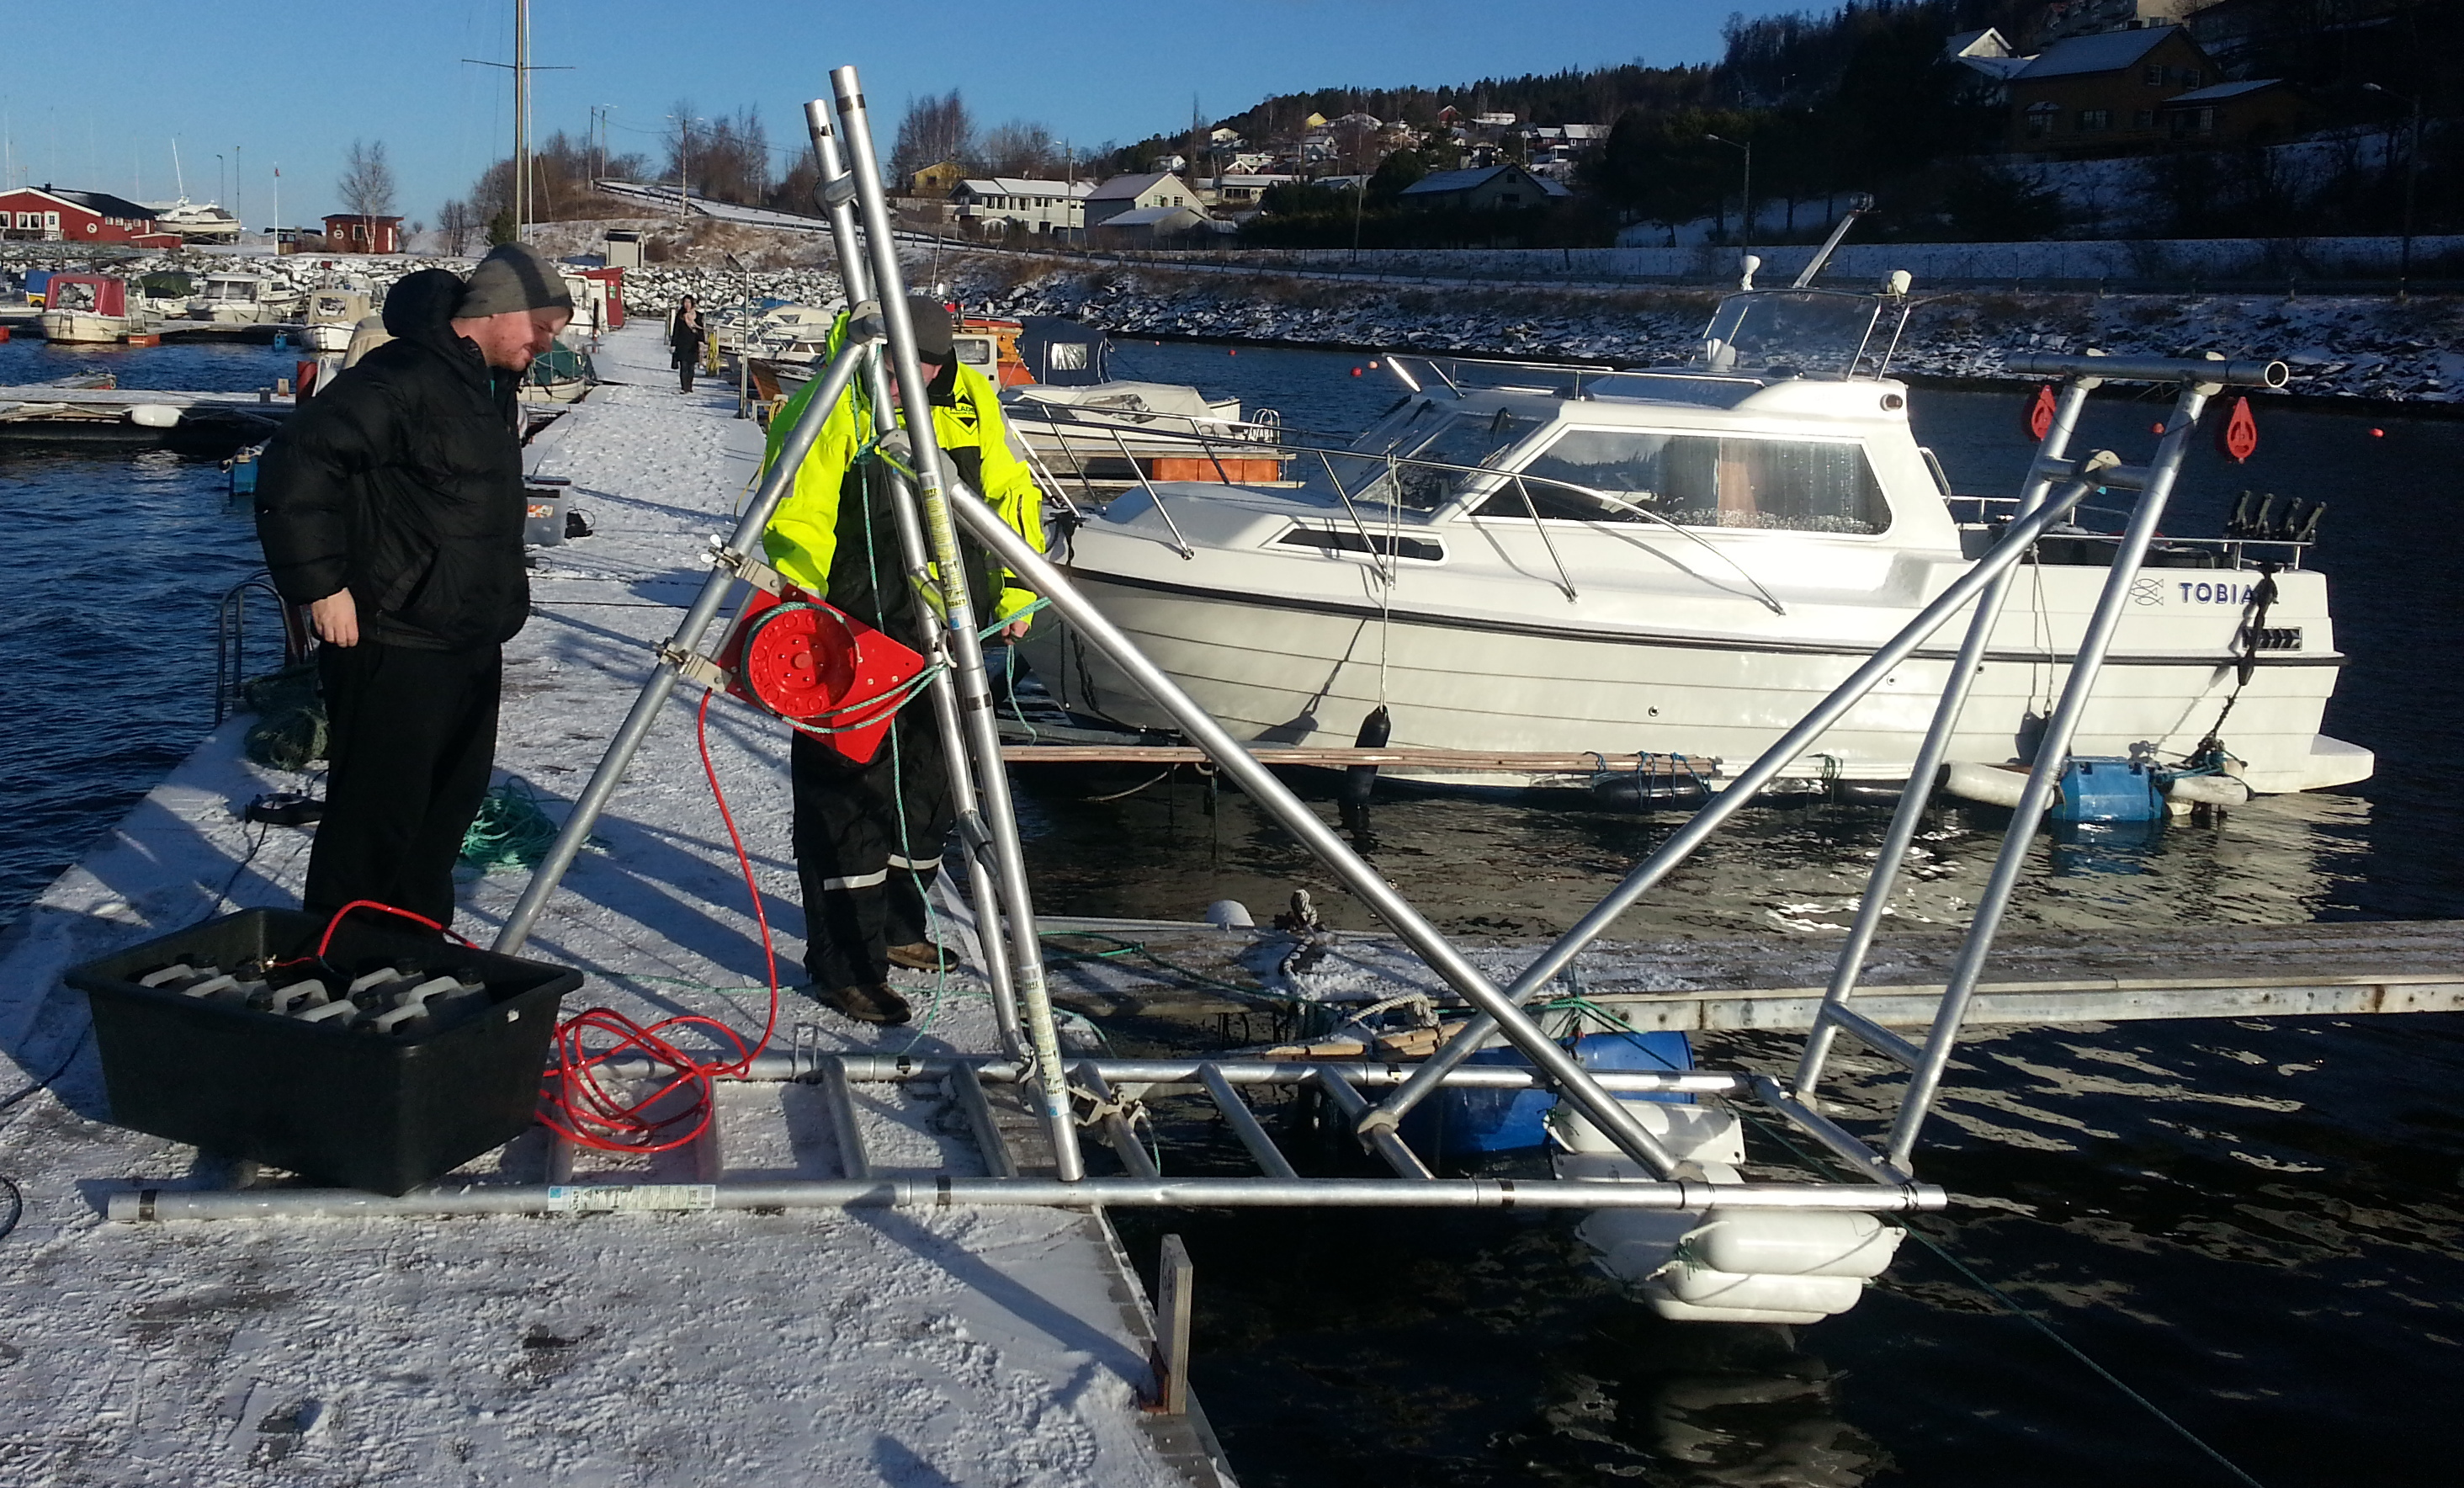
\includegraphics[width=0.9\textwidth]{rig1}
	\caption{Field test for \gls{sintef} using \gls{dvl}}
	\label{fig:test_dvl}
\end{figure}

\section{HD Video Test}

\begin{table}[htbp]
	\centering
	\begin{tabular}{ll}
		\toprule
			Net setup 					& Description  \\
		\midrule
			Reference					& Net in static position. No forced movement. \\
			Reference with movement		& Net lowered in front of the camera. \\
			Circular hole				& Net with a circular cut-out lowered. \\
			Vertical tear				& Net with a narrow vertical tear lowered. \\
			Horizontal tear				& Net with narrow horizontal tear lowered. \\
			L-shaped tear				& Net with horizontal L-shaped tear lowered. \\
			Growth						& Net with imitation growths lowered.\\
			Double sea-cage				& Two nets laid on top of each other.\\
		\bottomrule
	\end{tabular}
	\caption{Test setup, all at \SI{1.5}{\metre}}
	\label{tbl:test_setup}
\end{table}

\begin{figure}[htbp]
    \centering
    \subfloat[Circular Hole]{\label{fig:net_hole}{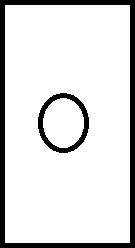
\includegraphics[width=0.3\textwidth]{net_hole}}} \hfill
    \subfloat[Vertical tear]{\label{fig:net_vertical}{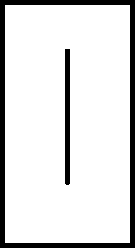
\includegraphics[width=0.3\textwidth]{net_vertical}}} \hfill
    \subfloat[Double net]{\label{fig:net_double}{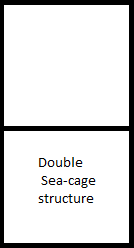
\includegraphics[width=0.3\textwidth]{net_double}}}
    \\
	\subfloat[L-shaped tear]{\label{fig:net_L_tear}{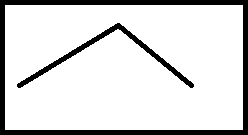
\includegraphics[width=0.45\textwidth]{net_l}}} \hfill
	\subfloat[Horizontal tear]{\label{fig:net_horize}{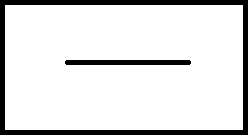
\includegraphics[width=0.45\textwidth]{net_horiz}}}
	\caption{Different net configurations with holes and tears, excluding normal single net. Images collected from \citet{sletta13}.}
	\label{fig:net_configs}
\end{figure}

\begin{figure}[htbp]
	\centering
	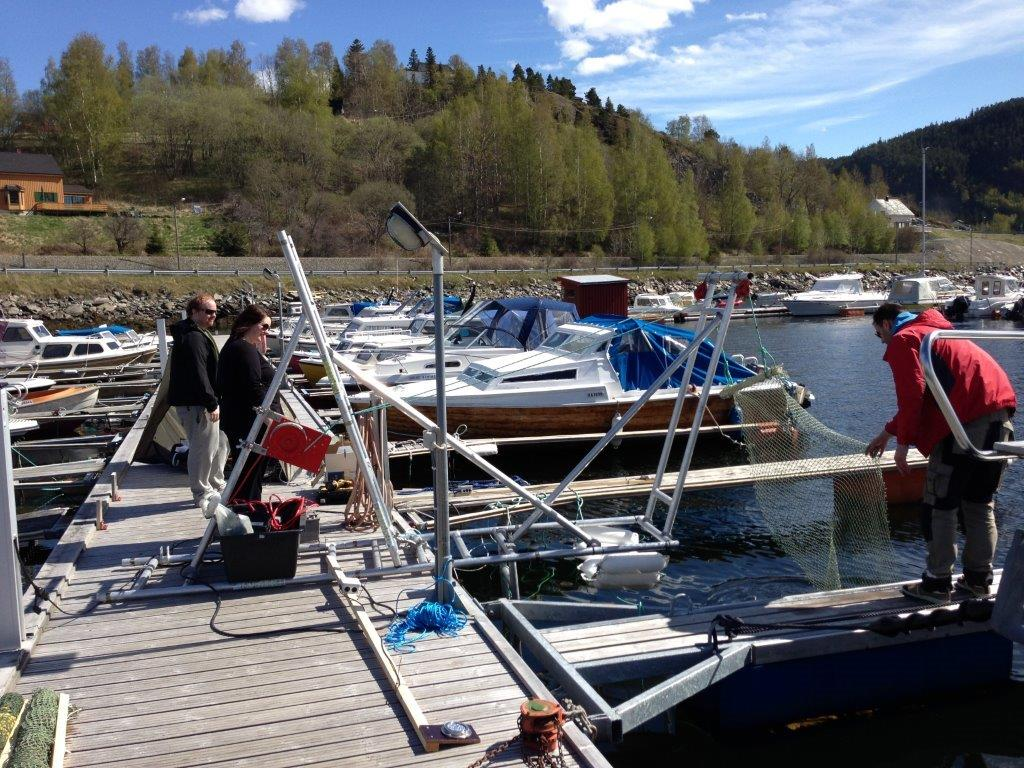
\includegraphics[width=0.9\textwidth]{rig2}
	\caption{Field test on a sunny day in May}
	\label{fig:test_hd}
\end{figure}

The rig was configured to mimic the approximate distance to the net 
in figure \vref{fig:sintef_not_1}. We were however not able to tilt the camera to 
an angle due to environmental constraint in a anchor chain situated below the camera.
We approximated the distance between the ROV and the net in figure \vref{fig:sintef_not_1} to be 
\SI{1.5}{\metre}. This lead to a the image in figure \vref{fig:test_hd_referanse}.

\begin{figure}[htbp]
	\centering
	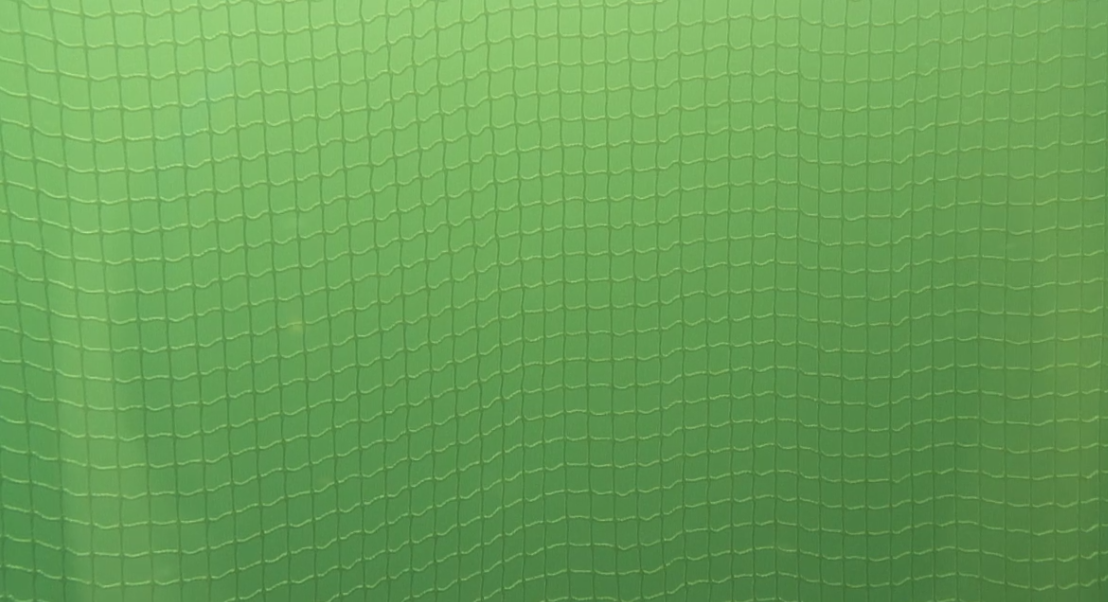
\includegraphics[width=0.9\textwidth]{hd_not_all}
	\caption{View of the net from \SI{1.5}{\metre}. This is the default distance for the rig used.}
	\label{fig:test_hd_referanse}
\end{figure}

Comparing image \vref{fig:test_hd_referanse} and \vref{fig:sintef_not_1}, it seems that the 
top row of masks is approximately the same in both images. Due to the tilt of the 
camera in image \ref{fig:sintef_not_1} we get a prominent vanishing point in that image. There 
are also some growing on the net in figure \ref{fig:sintef_not_1}, which of obvious reasons does not appear 
in figure \ref{fig:test_hd_referanse}.

\begin{figure}[htbp]
	\centering
	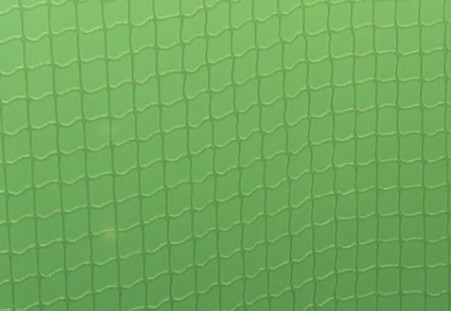
\includegraphics[width=0.9\textwidth]{hd_not}
	\caption{View of masks in the net at \SI{1.5}{\metre}. Digitally zoomed in post processing.}
	\label{fig:test_hd_clip}
\end{figure}

The test was done in accordance with the test patterns described in figure \vref{fig:net_configs}. 